% flotsam.tex
%
% Predrag created file              jun 20 2006
% $Author$ $Date$

\section{Flotsam}

\subsection{Template for KS equilibria discussion}

Ruslan L. Davidchack 3 Sep 2006:
http://www.math.le.ac.uk/people/rld8/temp/kse22explore.html homepage.


ES:{I observe pairs of real eigenvalues,
e.g. -58.3602685 and -58.3602681. As their absolute
value increases they differ even less.
I think it has to do with the linear part being the main
contribution to $\Mvar$ for higher modes, as well as
with treating real and imaginary components
as separate variables, which means it will appear twice.
        }

PC: {I think such contracting eigenvalues as -58.3602685 have no meaning.
Even if they are accurate eigenvalues of $\Mvar$,
what use is
$\ExpaEig_{radial} =  e^{\Lyap_p \period{p}} = e^{26\cdot58} = e^{1510}$.
        }

The \reqva (or travelling waves) appear to have a limiting propagation
velocity $c_{max} = \pm d/\period{}$.
To visualize them numerically,
start with a localized self-dual $u(x,0)$ such as
\[
u(x,0) = x e^{- x^2/2\sigma^2}
\,,
\]
with typical width $\sigma/2$ of order of typical wavelength
$\sqrt{2}$ (in $\tilde{L}$ system size units).
Time evolution of this  $u(x,t)$ is bracketed by two constant
pulses of apparently constant velocity $v=?$.
\RLD{generate figure, state $\sigma/2$, estimate $v$}
The notion of ``velocity''
is fuzzed up by the fact that the large peaks are preceeded
by smaller precursors.

PC: {Determine their velocity ANALYTICALLY?}

\underline{Stability of \KS\ equilibria:}{
% \label{exam:KSEquilStab}
% \index{Kuramoto-Sivashinsky equilibria}
\begin{table}
\caption[]{
Important \KS\ equilibria:
% in the antisymmetric solution
% space of the Kuramoto-Sivashinsky equation with periodic boundary % % % % condition,
% $ \nu =1$, $L=38.5$;
% their labels,
the first few stability exponents
%, with complex pairs written together.
}
\begin{center} \footnotesize
\begin{tabular}{@{}ccccc}
\hline %\br
$~S~~~$ & $~~~~\lambda_1 \pm \,i\,\theta_1$
                                & $~~~~\lambda_2 \pm \,i\,\theta_2$
                                        & $~~~~\lambda_3 \pm \,i\,\theta_3$
\\
\hline %\mr
${C_1}$    &{0.04422 $\pm \,i\,$0.26160}   &-0.255 $\pm \,i\,$0.431
&-0.347 $\pm \,i\,$0.463         \\
% ${C_2}$    &0.33053  & 0.097 $\pm \,i\,$0.243
% &-0.101 $\pm \,i\,$0.233        \\
\hline %\mr
${R_1}$   &{0.01135 $\pm \,i\,$0.79651} & -0.215 $\pm \,i\,$0.549
&-0.358 $\pm \,i\,$0.262        \\
%  ${R_2}$   &  0.33223  & -0.001 $\pm \,i\,$0.703
%  & -0.281 $\pm \,i\,$0.399      \\
\hline %\mr
${T}$     & 0.25480  & -0.07 $\pm \,i\,$0.645 &-0.264
\\
\hline %\br
\end{tabular}
\end{center}
\label{t:stationary}
\end{table}

{\em
spiraling out in a plane}, all other directions contracting


{\bf
Stability of ``center'' equilibrium
    }

linearized stability exponents:
\[ % \beq
(\lambda_{1}\pm\,i\,\theta_{1},\lambda_{2} \pm\,i\,\theta_{2}, \cdots)
    = (0.044 \pm \,i\,0.262\,,\,
        -0.255 \pm \,i\,0.431\,,\,\cdots)
\] %\eeq

The plane spanned by $\lambda_{1} \pm\,i\,\theta_{1}$ eigenvectors rotates with angular period
$\period{} ~\approx~2\pi/\theta_{1}=24.02$.
% 2*4*a(1)/0.26160 = 24.0182924586375

a trajectory
that starts near  the $C_1$~equilibrium point spirals
away per one rotation
with multiplier
$\ExpaEig_{\mbox{radial}}~\approx~\exp(\lambda_{1}\period{})=2.9$.
% 2*4*a(1)/0.26160*0.04422 = 1.062
% e(1.0620888) = 2.8924063421

each Poincar\' e section return,
contracted into the stable manifold by
factor of
{
$\ExpaEig_{2}\approx\exp(\lambda_{2}\period{})=0.002$
}
%2*4*a(1)/0.26160*(-0.255) = -6.12466
%e(-6.12) = .0022


The local Poincar\' e return map is
{\em
in practice $1-dimensional$
}
    } %end \example{{Stability \KS\ equilibria


% Staring at the solution
% as it evolves in time we should start getting a glimpse of the
% repertoire of the spatiotemporal patterns charcterizing
% the turbulent dynamics.

Many of the \rpo s can be constructed from segments corresponding to
close approches to some of these equlibria.

\subsection{Numerical methods}

Shroff and Keller\rf{shroff:1099}
``The Recursive Projection Method" (RPM)
might be of interest to us in numerical work.
RPM stabilizes fixed-point iterative
procedures by computing a projection onto the unstable subspace.
On this subspace a Newton or special Newton iteration is performed,
and the fixed-point iteration is used on the complement.
The method is effective when the dimension of the unstable subspace
is small compared to the dimension of the system.
Examples are presented for computing unstable steady states.
The RPM can also be used to accelerate iterative procedures when
slow convergence is due to a few slowly decaying modes.

PC also has 2 hard-copy, rather readable
old proceedings reprints by Keller\rf{Keller77,Keller79}.
There are some readable words about homotopy methods in
\refref{AllgGeorg88}.

{\Rpo s} were missed in earlier
previous \KS\ investigations%
\rf{Christiansen:97,Lan:Thesis}
which focused on the antisymmetric subspace, where translational invariance
is broken.

\subsection*{Papers that cite \refref{Christiansen:97}}

Read these papers:

Misiurewicz and Zgliczynski\rf{misiurewicz-topological}

Zgliczynski and et al.\rf{zgliczynski-rigorous}

Zimmermann\rf{zimmermann-global}

\subsection*{V. Lopez:
        {\Rpo s} of the Complex Ginzburg-Landau Equation}

        Recently
 Viswanath found such in plane Couette.

As far as the discussion about ``drift" is concerned:
In presence of continuous symmetries (for PC, streamwise and
spanwise translations) one should be searching for
{\reqva} and
{\rpo s} - they are most likely more important than
the stationary equilibria and spatially periodic orbits.

I like {\rpo s} paper\rf{lop05rel} by
Vanessa Lopez\rf{lopezLink},
%        http://www.cse.uiuc.edu/$\sim$vlopez:
``Relative Periodic Solutions of the Complex Ginzburg-Landau Equation"

% [From siads\@siam.org  Dec 22 2004]:
% willing to review this manuscript for Dwight Barkley.

A method of finding {\rpo s} for differential equations with
continuous symmetries is described and its utility demonstrated by computing
{\rpo s} for the one-dimensional complex Ginzburg-Landau
equation (CGLE) with periodic boundary conditions.  A {\rpo} is
a solution that is periodic in time, up to a transformation by an element of the
equation's symmetry group.  With the method used, {\rpo s} are
represented by a space-time Fourier series modified to include the symmetry
group element and are sought as solutions to a system of nonlinear algebraic
equations for the Fourier coefficients, group element, and time period.
{\Rpo s} found for the CGLE exhibit a wide variety of temporal
dynamics,
with the % sum of their positive Lyapunov exponents varying from 5.19 to
% 60.35 and their
unstable dimensions from 3 to 8.

15 Sep 2004, Predrag Cvitanovic:
All of your {\Rpo s} have many unstable
eigendirections. Do you know that there exist no other solutions with a
lesser number of unstable directions (let's say only one)?

--vanessa:
I do not know of any proof that shows that there are no solutions with a
lesser number of unstable directions.  I did not find any solutions with
just one or two unstable directions, but at this point I cannot say
whether that is an indication that there are none or simply that
the procedure I used only identified solutions with 3+ unstable
directions.

15 Sep 2004, Predrag Cvitanovic:
Periodic solutions are usefull if they are embedded into a chaotic
attractor. Do you have any measure of whether the typical solutions of
CGL, your parameter values, come close to any of the solutions that you
have found? If the periodic orbit is embedded into a chaotic attractor,
typical soultion visits it infinitely often, infinitesimally close.

--vanessa:
This is something that I have not examined in detail.  I have observed (using
the ``naked eye") that the time evolution of typical trajectories (when viewed
by plotting the real versus imaginary part of A(x,t) at different times, as in
Figures 3,5,7 from the paper) sometimes resembles that of the first solution
found (i.e., the patterns displayed in Figure 3). (The first solution
found also happened to be the solution to which the solver I used
converged to most frequently.)  But I do not have a
quantitative measure of this ``resemblance".

After talking to Lopez at SIAM DS05 meeting: I do not think
her \rpo s are the dynamically important ones, so the problem remains wide open.

I read through
Vanessa Lopez's paper (clearly a summary of a PhD thesis), and while I
a like {\rpo s}, I am very worried about the general drift
of the paper.

As I cannot tell how exhaustive is her set of numerical solutions, I do
not know what to make of them - like ZG, she gets all of them with a large
number unstable dimensions. Presumably none of them are close to the
asymptotic inertial manifold. More worrisome still, she uses ZG to
``average" over periodic orbits. That is regrettable - I hoped I would
never see that stuff again. Dettmann and I tried to get Zoldi to
derive this for us, and Mainieri actually hired him at Los Alamos to learn
how this works. We are all convinced that it makes no sense whatsoever.
Regrettably Lopez used the nonsensical formulas of Zoldy, so that will
just keep confusing future readers.
She is in computer science, so cannot
blame a graduate student for trying a formula published in Phys Rev Lett.


If she is right and CGL at her parameter values does not contain
(relative) periodic orbits with 1 or very few unstable directions, we can
kiss the ``minimal instability principle" goodbye.

The
periodic orbits
did not capture the chaotic dynamics of the system. In fact, in the full
space I believe that the {\rpo s} are the more commonly
encountered objects in the \statesp, just as the quasi-periodic motion is a
more frequent occurrence on an invariant torus. In a system with continous
symmetry, any orbit corresponds to a continous family of orbits, so the KS
system with periodic boundary condition is born on some kind of torus. We can
either reduce the system so that the continuous symmetry does not exist, or
study {\rpo s}. {\Rpo s} correspond to periodic
orbits in the reduced system. I don't know how to reduce the KS system in a
pretty way.


        Here we discuss these continuous symmetries as
a small-step limit of discrete symmetries:

\begin{enumerate}
\item
        symmetries of 3-disk
\item
        $C_n$ symmetry of $n$-slice pizza without reflection symmetry
\item
        Fourier analysis of periodic lattices
\item
        running modes in periodic lattice deterministic
           diffusion
\item
    celestial {\rpo s}
\end{enumerate}

The reading material for 1)-3) is on
http://www.cns.gatech.edu/courses/chaosSpring06

In my \KS\ work with Christiansen, Putkaradze and Lan we
had excluded them ``by hand", by concentrating only on the space of
antisymmetric solutions. That is not good physics, as perturbations off
them mix into the full space of asymmetric solutions.

\subsection{Thomas J. Bridges: [2006]  Degenerate relative equilibria,
           curvature of the momentum map, and homoclinic bifurcation}

www.maths.surrey.ac.uk/personal/st/T.Bridges/TJB.html

A relative equilibrium (RE) is a solution which travels along an orbit of the symmetry group
at constant speed. They are pervasive in applications such as celestial mechanics, molecular
dynamics, mechanical systems, and fluid mechanics. An introduction to the theory of RE can
be found in Chapter 4 of Marsden [14].

[14] J.E. Marsden. Lectures on Mechanics, London Mathematical Society Lecture Notes 174,
Cambridge University Press (1992).




\subsection{F Laurent-Polz: {\Rpo s} in point vortex systems}

Testing bibtex - these should exist:
\refrefs{Laurent-Polz04,lop05rel,McCordMontaldi}
\refrefs{Vanderb,Wulff00}

We give a method to determine {\rpo s} in point vortex systems: it consists mainly

into perform a symplectic reduction on a fixed point submanifold in order to obtain
a two-dimensional reduced \statesp. The method is applied to point vortices systems
on a sphere and on the plane, but works for other surfaces with isotropy
(cylinder, ellipsoid, ...). The method permits also to determine some
{\reqva} and heteroclinic cycles connecting these {\reqva}.

    {\Reqva} are orbits of the symmetry group action which are in-
variant under the flow, this corresponds here to motions of point vortices which
are stationary in a steadily rotating frame.
 The existence and nonlinear stability
of {\reqva} formed of three vortices have been studied respectively in
[KN98] and [PM98].

Periodic orbits on the sphere were determined in [ST,To01] thanks to the
following method: they reduced the system to two-dimensional systems by a
symmetric reduction (using some finite subgroups of $SO(3)$); the computation
of the dynamics on the reduced spaces permits then to determine periodic orbits.
Our paper is devoted to transpose that method to determine {\rpo s}.
To this end, we combine a symmetric reduction together with a symplectic reduction.

[Third Referee's Report Dr Newton]:
The manuscript considers {\rpo s} in point vortex systems
that arise from splitting {\reqv} configurations. It more
comprehensively treats problems of the type considered in Souliere and
Tokieda (2002) and Tokieda (2001). It is a very nice paper.

Angel Duran,
Numerical Integration of Hamiltonian
Relative Periodic Solutions. A First Approach
http://www.math.human.nagoya-u.ac.jp/scicade05/
% angel@mac.uva.es

    [1] B. Cano and A. Duran, A technique to improve the error propagation when inte-
grating relative equilibria, BIT 44(2004) 215-235.
    [2] A. Duran and J.M. Sanz-Serna, The numerical integration of relative equilibrium
solutions. Geometric theory, Nonlinearity 11(1998) 1547-1567.
    [3] E. Hairer, Ch. Lubich and G. Wanner, Geometric Numerical Integration. Structure-
Preserving Algorithms for Ordinary Differential Equations, Springer Series in Comput.
Mathematics, Vol. 31, Springer-Verlag 2002.

\PC{probably cite:
\rf{Creagh91}
    % author = {Creagh, Stephen C. and Littlejohn, Robert G.},
    % title = {Semiclassical trace formulas
    % in the presence of continuous symmetries},
\rf{Creagh92}
    % author = {Creagh, Stephen C. and Littlejohn, Robert G.},
    % title = {Semiclassical trace formulas
    % for systems with non-Abelian symmetry},
\rf{robb}
    % author = {Robbins, Jonathan M.},
    % title = {Discrete symmetries in periodic-orbit theory},
\rf{mta}
    % author = "Abraham, Ralph and Marsden, Jerrold E. and Ratiu, Tudor",
    % title =  "Manifolds, Tensor Analysis, and Applications",
\rf{ViswanathPC06}
    % author = {Viswanath, Divakar},
    % title = {Recurrent motions within plane Couette turbulence},
\rf{Wulff00}
    % author = {C. Wulff},
    % title = {from relative equilibria to relative periodic orbits},
    }

\bigskip

Reduction of the dynamics to the fundamental domain is particularly
useful in periodic orbit calculations, as it simplifies symbolic dynamics
and improves the convergence of cycle expansions\cite{CvitaEckardt}.

some of the \po s will
halve their period, and symmetric pairs will be eliminated.

\subsection*{Antisymmetric subspace}
%\label{s:AntisymmSubspFlot}

Fix the  Poincar\'e section to be the hyperplane
$\Re a_1=0$. We integrate \refeq{expan} with the initial
 conditions
$\Re a_1=0$, and arbitrary values of the coordinates  $a_2, \ldots, a_N$, where
$N$ is the truncation order.  When $\Re a_1$ becomes
$0$ the next time,  the coordinates  $a_2, \ldots, a_N$ are mapped
into $(a_2', \ldots a_N')=P(a_2, \ldots, a_N)$, where $P$ is the  Poincar\'e
map. $P$ defines a mapping of a $N-1$ dimensional hyperplane into itself.
Under successive iterations of  $P$, any trajectory
approaches the attractor ${\cal A}$, which itself is an invariant
set under $P$.

A trajectory of
 (\ref{expan}) can cross the plane $a_1=0$ in two possible ways:
 either when
$\dot{a_1}>0$ (``up'' intersection)
or when  $\dot{a_1}<0$ (``down'' intersection),
 with the ``down'' and ``up'' crossings
alternating.
It then makes sense to define the  Poincar\'e map $P$ as a transition between,
say, ``up'' and ``up'' crossing.
With  Poincar\'e section defined as the ``up-up'' transition,
it is natural to define a ``down-up'' transition map $\Theta$. Since
$\Theta$ describes the transition from down to up (or up to down) state,
the map $\Theta^2$ describes the transition  up-down-up, that is
$\Theta^2=P$.


\subsection*{Heteroclinic and homoclinic connections}
%
% from \Chapter{KS}{12Jun2004}{Steady solutions of KS equation}
% Lan                                            8Jun2004

\PC{either drop this, or credit \refref{Lan:Thesis,LanCvi07}
    if we need it
   }
\KSe\ \refeq{eq:stdks} has an exact heteroclinic solution
\beq
u=a_1 \tanh(kx)+a_2 \tanh^3(kx)
\label{eq:ksexa}
\,,
\eeq
for the specific value $c=-\frac{30}{19}k^2(304\,k^4-40\,k^2+1)$ where
\[
a_1=60\,k^3-\frac{30}{19}k
    \,,\qquad
a_2=-60\,k^3
    \,,\qquad
k^2=11/76 \mbox{ or }
k^2=-1/76
\,.
\]
When $k^2=-1/76$, the hyperbolic tangent becomes ordinary tangent and there are poles on
the real axis. Near the singularity $x_0$, $u$ blows up as
\[
u(x) \approx \frac{-60~}{(x-x_0)^3}
\,.
\]
All blow-up solutions possess singularities of the same type\rf{ksham95}.

\bigskip

Perhaps there is some way of plotting the unstable manifolds too. If
there is only one unstable direction (in the full Fourier space
representation), the corresponding eigenvector is a unique loop function
$h[s] =  h(u(s),v(s),w(s))$ in the $(u,v,w)$ space, and the unstable manifold
$U$ is swept out by evolving in time the perturbed loop
$L[s] + \delta h[s] =  L(u(s),v(s),w(s)) + \delta h(u,v,w)$
$\to$ $L[s,t]$.
Complex eigenvector defined unstable manifold plane seems
harder to visualize;  It would be interesting
to look at heteroclinic connections in the $(u,v,w)$ space, as
behavior of higher-frequency modes in Fourier reps is a bit
hard to get used to.

\bigskip

Note also that in your L22-long.eps one seems
to come quite close to \EQV{2}~\eqv, so it might be a very dominant
influence on the strange attractor dynamics


There appears to be a heteroclinic connection from \EQV{2}
{\eqv}
unstable spiral out straight into \EQV{3}~{\eqv}
$\period{} = 76.6$ \rpo\ seems like a close-by
relative of this.
That also means that the relative shift between the two {\eqva} is
fixed, as far as this connection is concerned.

KS symbolic dynamics will
serve as a test bed for developing the
same for PCF, and for applications of the new
trace formula with continues symmetries.

% "Ruslan L. Davidchack" <rld8@mcs.le.ac.uk>, 2 Nov 2006
%
Isn't there another $ \EQV{2} \to \EQV{3} $ heteroclinic
from the same point on  \EQV{2} circle that connects to a different point on
\EQV{3} circle?


\bigskip

It is imperative that we start using the discrete symmetries, and only 1/2
of trajectory when it is selfdual.
\EQV{1}, \EQV{2} and \EQV{3} and unstable eigenvectors
we care about all happen to sit in the antisymmetric subspace
(recheck...), so connections should reflect these multiplicities. We have
one $\EQV{2} \to \EQV{3}$ and $\EQV{2} \to \EQV{2}$ (shift by $L/4$).

The \rpo\ {\nameit}55 travels between the 2-\eqv\  and
2-\eqv\ shifted,
with period and shift
$\period{p}=55.5953\,,\ d=5.24725$
Compared to $L/4 = 5.5$
this is nice, but why not close to periodic after 2nd return? Why 4th return?

The {\nameit}2 {\eqv}
captures qualitatively the mean velocity frame \rpo\ {\nameit}55 shape,
which follows the
{\eqv} for most of the time, except for a quick swing where it
sidesteps by $d/4$, just as it does in \reffig{f:rpo55}.

\Rpo\ {\nameit}55 looks similar to Davidchack's  orbit
of period
$\period{p}=47.64$ and $d=5.6759$. The period appears to depend on how
many times the orbit manages to spiral around the \eqv.
For {\nameit}55 that appears to be
1.5 times per period, rather than 2. This would led as
to
think there is a family of \rpo s along with a 3rd unit eigenvalue of
$gJ$,
but such does not exist.
So there has to be a selection mechanism corresponding to
reaching or missing the neighborhood of an \eqv\  point starting from
the neighborhood of the other.

The $u$ space time evolution \reffig{f:rpo55u} % rpo22-55-4-u.eps
is plotted with the same starting instant,
so one can also track also the spatial profile $u$ in parallel with
the Fourier space projections.

So it is almost impossible to see \reffig{f:rpo55}(b) %rpo22-55-4-cm.eps
in \reffig{f:rpo55}(a) % rpo22-55-4.eps.
I can see 4 periods in \reffig{f:rpo55}(a), %po22-55-4.eps,
but not in \reffig{f:rpo55}(b) %rpo22-55-4-cm.eps
where it comes back only after full period $\period{p}=55.6$.

It still seems that it could be made relative periodic
(modulo a reflection symmetry?)
in $\period{p}/4=55.6/4=13.9$? That would be OK
-
by symmetry the figure 8 connecting
2 symmetric {\eqva} could consist of 4 identical segments: from
{\eqv} A to midplane, then reflected version of the same to SA, and
back again.

The two {\eqva}
capture qualitatively the mean velocity frame \rpo\ {\nameit}55 shape,
which follows the
{\eqv} for most of the time, except for a quick swing where it
sidesteps by $d/4$, just as it does in \reffig{f:rpo55}.

Please also plot it in plane, chose small Fourier coefficients
 which respect the $x \to -x$ symmetry of \KSe.
Then the symmetry of 2 mean velocity
{\eqva} and self-dual symmetry of \rpo\ {\nameit}55 will be explicit.

Eigenvalues of \rpo\ {\nameit}55 $g\jMps$: are
\\
$(-57.17,  1, 1, -0.500, -0.012, \cdots)$ .
%
%  Eigenvalues of the Jacobian without rotation
%  84.15, -33.86 + 28.94 i, c.c. , 0.48, 0.00019
% no good - missing marginal ones

plots:
  76 rpo60fm23.jpg  \\
 909 rpo60fm23.emf  \\
% Ruslan L Davidchack,  10 Jul 2006
the 55 rpo, or whichever seems easiest to explain:
$\period{} = 59.89$,
$c_p = \shift_p/\period{p}= ?$

$(\ExpaEig_i e^{\pm i\theta_i})=
(
\\
 -27.03397007874626,
\\
   9.34426620337976,
\\
   1
\\
   1
\\
  -0.05018967056231,
\\
   0.00015065158255,
)$

The eigenvectors
indicate that an amplitude mode comes paired with the
group shift-invariant mode $\ExpaEig_4 =1$. It probably says that
the amplitude $|u_k|$ of the associated can be easily perturbed (think of
a large system: $|u(x)|$ can be easily deformed by long wavelength
perturbations. This \underline{must} be understood. Proposal:

There are two
marginal eigenvalues, one for time translation, one for
rotational invariance.
The sign of $\ExpaEig_{1}=-57$ says this is a Moebius-kind orbit,
inverse hyperbolic.
Stability exponent
 $\eigExp[1]=0.07$ says that this neighborhood is much less repelling than
the central {\eqv} A, a better candidate for being embedded into the
ergodic attractor.

The \rpo\ initial condition is
so accurate the orbit in \reffig{f:rpo55}(b)
start visibly deviating after retracing the loop 6.5 times.
% the largest unstable multiplier is
% $-57.17$ per period of the orbit - error would grow to $\approx 60^7
% = 2,800,000,000,000$.

For the \rpo s the accuracy of Jacobian depends
on the time step size, and long runs are needed to refine the results

For a numerical check of the \rpo\ stability eigenvalues,
used two inital
points along an unstable eigenvector $\jEigvec{1}$
at radial distance  $\approx 10^{-4}$ from the \eqv\ {\nameit}2,
and the initial inter-point separation $\Delta(0) \approx 10^{-5}$.
Integrated for time equal to the period $\period{p}=26.3556$ as calculated from
the \jacobianM\ and computed the leading Lyapunov exponent from the ratio of
final to initial distance
$\Lyap= \frac{1 }{ \period{}}\ln( \Delta(\period{})/\Delta(0))$.
Get
$\Delta(\period{})/\Delta(0) =39.01$,
$\Lyap=0.13902$, in agreement with the \eqv\ {\nameit}2
expanding eigenvalue $\Lyap=0.13904$
\[
\ExpaEig_{radial} =  e^{\Lyap \period{}} =38.99
\,.
\]

% Ruslan L Davidchack,  10 Jul 2006
The orbit RLD found has period 60
rather than 55.  Because it comes so close to the steady states,
this is probably a numerical precision error.
\\
plots:
 180 rpos1.jpg  \\
1594 rpos1.emf  \\


Rewrite Fourier modes as $u_k(t) = e^{r_k(t) + k(\theta_k(t))}$, study
dynamics and Jacobinas in the $\dot{r_k},\dot{\theta_k})$ representation.
\nameit 2 and \nameit 3 \eqva\ are nearly cirlces in this representation - higher
modes will not wind wildly if represented by $\theta_k(t)$? Kind of WKB
representation.

period 77 rpo jumps between the two steady states.
\\
plots:  \\
  84 rpo77fm23.jpg  \\
1133 rpo77fm23.emf  \\
 176 rpos2.jpg  \\
1594 rpos2.emf  \\


\bigskip

%%%%%%%%%%%%%%%%%%%%%%%%%%%%%%%%%%%%%%%%%%%%%%%%%%%%%%%%%%%%%%%%
\begin{figure}[t]
\begin{center}
(a) \includegraphics[width=5.0cm]{figs/1wSteadyE.eps}
\hspace{0.1in}
(b) \includegraphics[width=5.0cm]{figs/1wSteadyP.eps}
\end{center}
\caption{
(a) \EQV{1} in $(u,u_x,u_{xx})$ representation along with the eigenvectors of the equilibrium
point $(\sqrt{c},0,0)$. The blue line represents the unstable eigen-direction.
(b) \EQV{1} projected along the above eigenvectors.
% $\tildeL=3.5014$, $N=64$ complex modes truncation.
}
\label{f:1wSteady}
\end{figure}


%%%%%%%%%%%%%%%%%%%%%%%%%%%%%%%%%%%%%%%%%%%%%%%%%%%%%%%%%%%%%%%%
\begin{figure}[t]
\begin{center}
    \includegraphics[width=0.18\textwidth]{figs/rpo22-55-4-u.eps}
\end{center}
\caption{
 The \rpo\ {\nameit}55 in $u(x,t)$ representation.
        }
\label{f:rpo55u}
\end{figure}
%%%%%%%%%%%%%%%%%%%%%%%%%%%%%%%%%%%%%%%%%%%%%%%%%%%%%%%%%%%%%%%%%%




This observation can be heuristically motivated as follows.
\PC{this argument keeps worrying me: there are lots of solutions, like
$u=0$, that are {\eqva}, but isolated -
they are noplace near asymptotic dynamics.
Do they belong to the invariant manifold?
   }
Equilibria are solutions valid for all times, and are thus points
on the finite-dimensional compact inertial manifold\rf{infdymnon}.
Finite dimensionality of the inertial manifold
bounds the size of Fourier components of all solutions.
This
compact inertial manifold and the dynamics on it can be
described by analytic functions of a finite number of Fourier modes.
\PC{explain the theory; say that in practice it is useless}
On a finite-dimensional compact manifold,
an analytic function can only have a finite number
of zeros. So the {\eqva}, {\ie},
the zeros of a smooth velocity field on
the inertial manifold, are finitely many.
The number of {\eqva} increases exponentially with $L$,
\PC{give reference for ``exponential growth''}
for infinite system size $L \to \infty$,
there are infinitely many {\eqva}.
\PC{is there a reference where this is explained?}

\bigskip

consult often
\\
        www.math.le.ac.uk/people/rld8/temp/kse22explore.html
\\
we have to systematize it, and
construct the complete cage of heteroclinic $\EQV{1}$, $\EQV{2}$, $\EQV{3}$,
$\REQV{+}{1}$,
$\REQV{-}{1}$,(?)
connections, \underline{divided} by the $u(x) \to - u(-x)$ symmetry.

The hope is that $\EQV{1}$,
$\REQV{+}{1}$,
$\REQV{-}{1}$,(?) are transient, and \rpo\ symbolic
dynamics (\underline{divided} by the $u(x) \to - u(-x)$ symmetry, otherwise
unnecessarily messy) comes from the closed loops on
the $\EQV{2}$,$\EQV{3}$ part of the cage.


It is very unlikely that a single 1-$d$ Poincar\'e section,
can do the job, previous work\rf{Lan:Thesis,LanCvi07}
always needed several sections.

The idea is that the local unstable plane gives 2 coordinates, the
least contracting direction (or one of a complex pair) gives the 3rd.

We need to construct the backbone of heteroclinic connections
first. They are not like 3-$d$ R\"ossler and Lorenz examples:
here one spirals out,
then spirals in - hopefully there will be intelligent Poincar\'e sections
transverse to initial \EQV{2} (or {\EQV{3)} unstable manifold, mapping onto
Poincar\'e sections of trajectories leaving again
the next \EQV{3} or \EQV{2} unstable manifold.

% Ruslan:  10 Jul 2006
%
% 119 KB     "long_orbit.jpg"
%  88 KB     "steady_states1.jpg"
%  84 KB     "steady_states2.jpg"
% 197 KB     "rpos1.jpg"
% ----------------------------------------

For all spatial plots color axis $u \in [-3, 3]$ is the same,
same time units and spatial width $L$.
For the steady states the magnitude of the \EQV{2} is quite
a bit smaller than that of the \EQV{3}.

On the
    $[a_?,a_?]$ plane
    the $\sigma x = -x$ symmetry of \KSe\ is explicit.


steady\_states1.jpg shows the numerical evolution and, since the
traveling wave is very unstable, it disappears after awhile.
The numerically exact solution is plotted in steady\_states2.jpg

rpos1.jpg is attached as a sample.

As it looks, will not help us with partitioning, it seems, unless there is
a trajectory that hits the contracting direction - maybe
( -0.11941393,0)
head on.

Might want to look at this blowup in
the \EQV{2} slowest contraction
$   ( -0.08402656 \pm i 0.16019413)$
complex eigenvectors plane, check whether the
spiralling rotation agrees with the real/imaginary parts of eigenvalues.

Question is still - why does all of the unstable manifold of
\EQV{2}~\eqv\ go back
into
\EQV{2}~\eqv?


%%%%%%%%%%%%%%%%%%%%%%%%%%%%%%%%%%%%%%%%%%%%%%%%%%%%%%%%%%%%%%%%
\begin{figure}[t] \label{f:neighborhood2w}
\begin{center}
(a) 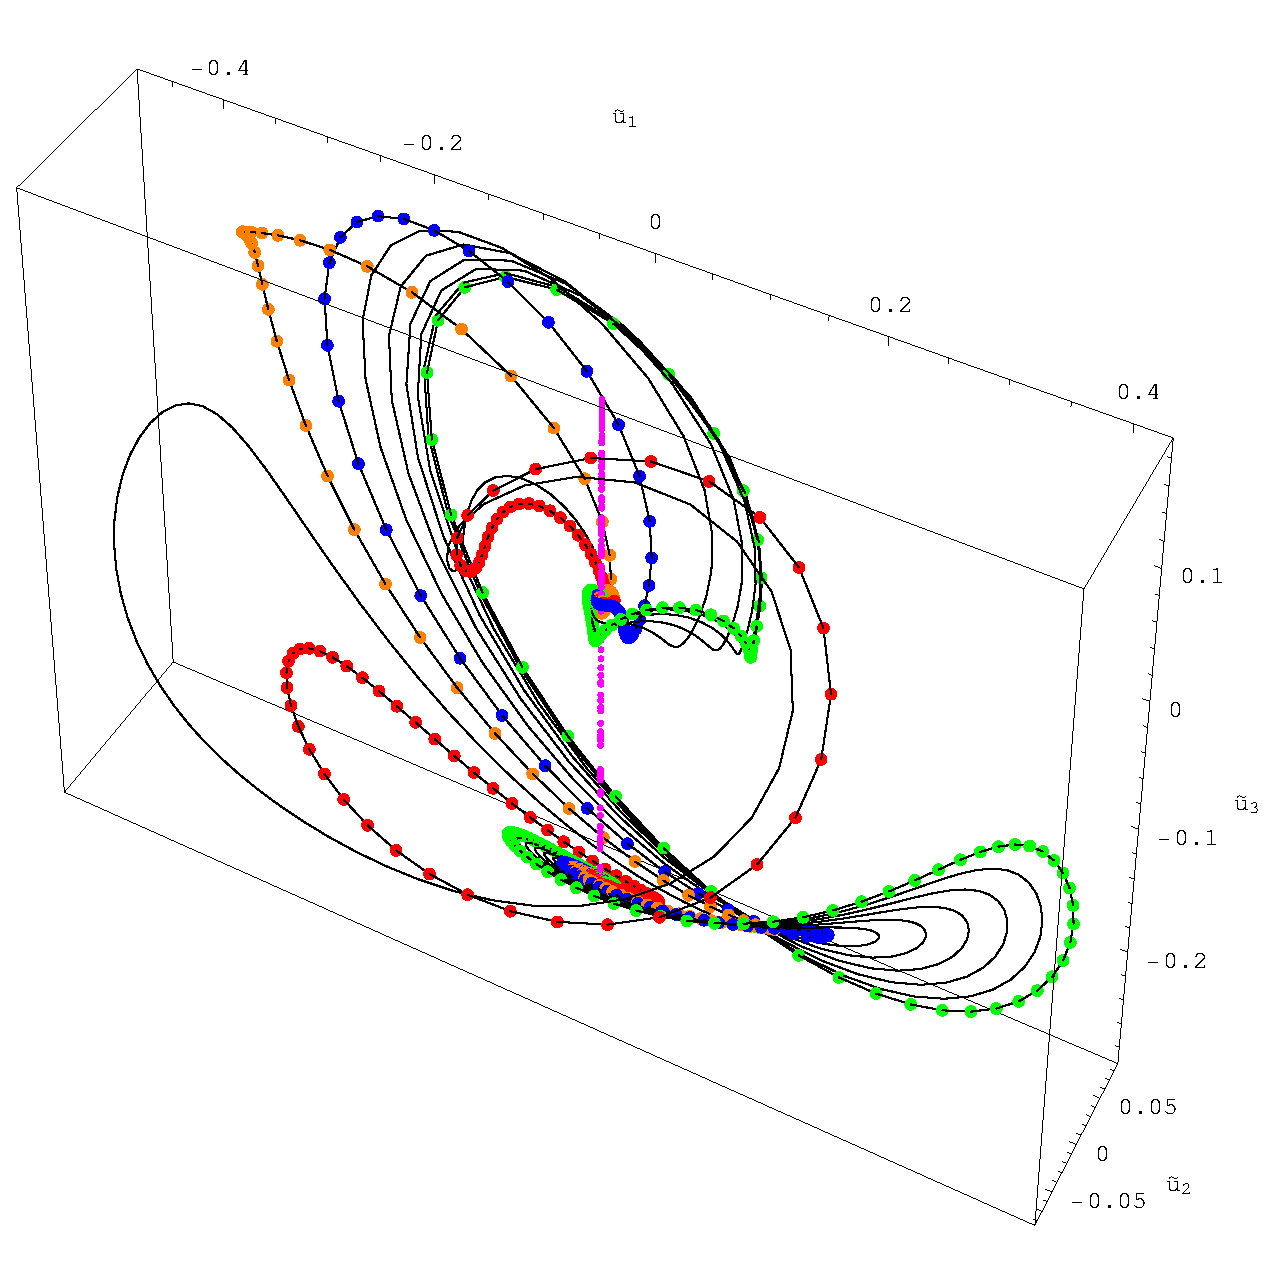
\includegraphics[width=5.0cm]{figs/L22-2w-UnsMan.eps}
\hspace{0.1in}
(b) \includegraphics[width=5.0cm]{figs/L22-2w-UnsMan-BlowUp.eps}
% (b) \includegraphics[width=4.0cm]{figs/L22-2w-R.eps}
\\
(c) \includegraphics[width=5.0cm]{figs/L22-2w-3w-UnsMan.eps}
% (c) \includegraphics[width=4.0cm]{figs/L22-2w-G.eps}
\hspace{0.1in}
(d)  \includegraphics[width=5.0cm]{figs/L22-2w-3w-detail.eps}
% (d) \includegraphics[width=4.0cm]{figs/L22-2w-B.eps}
\end{center}
\caption{
 Trajectories with initial conditions on the unstable subspace of
 the \EQV{2}~\eqv.
 (a) The coordinates $\tilde{u}_1$ and $\tilde{u}_2$
 are along the directions defining the unstable subspace
 and $\tilde{u}_3$  is along the real part of the eigenvector
 corresponding to the eigenvalue $-0.271122+ i\, 0.356307$.
The purple points represent the continuous family
 of
\EQV{2}~\eqva.
% Green curve belongs to \reffig{f:rpo55}(b) % rpo22-55-4-cm.eps
% rather than to  \reffig{f:rpo55}(a), % rpoEq22-55-4.eps?
(b) blowup of ``homoclinic'' descent of the unstable manifold
back into \EQV{2}~\eqv, shifted by
$L/4$.
(c) blowup of ``heteroclinic'' connection from
\EQV{2} \eqv\ to \EQV{3} \eqv, with shift
$L(1/3-1/4) = L/12$
\PCedit{(? check)}
to the neighborhood of the point near which the
unstable manifold of the
\EQV{2} \eqv\ splits. The blue points
represent the
\EQV{3} {\eqv} family.
The descent is along the eigenvector of $\Lyap_4= 0.413$,
\ESedit{(checked)}
and splitting
occurs along one of the
$\Lyap_1=\Lyap_2=0.0933$
unstable directions of the \EQV{2}~{\eqv}.
\ESedit{(checked)}
(d) same as (c), closer to the \EQV{3}~{\eqv}.
The eigendirections corresponding to $\Lyap_1$
and $\Lyap_4$ are shown in purple.
}
\end{figure}
%%%%%%%%%%%%%%%%%%%%%%%%%%%%%%%%%%%%%%%%%%%%%%%%%%%%%%%%%%%%%%%%%%

\underline{1-\reqv\  (traveling wave).}
% Ruslan L Davidchack,  10 Jul 2006
There is a pair of {\reqva}
${\nameit}1L$,
${\nameit}1R$
(traveling waves), dual under the
$u(x) \to -u(-x)$ symmetry. They are
determined numerically by
adiabatic continuation from a smaller system size
$L~\approx 12$,
where they are stable, to $L=22$
where their velocity is atypically large, $c=0.737$,

Their exponents are:
\\
$\Lyap_i \pm \theta_i =
(
\\
  0.1156222 \pm 0.817289,   \\
  0.033663 \pm 0.418909,    \\
 0.0                    ,   \\
 -0.245729                    , \\
 -0.321321 \pm 0.98126,
\cdots
)$

The pair of \reqva\
${\nameit}2L$,
${\nameit}2R$
exists for larger system sizes, but does not continue
adiabatically\rf{KNSks90} down to $L=22$.


\section*{Numerical searches for \reqva\ and \rpo s}

% \subsection{Newton's method for determining \reqva}


The problem one faces with high-dimensional flows is
that their topology is hard to
visualize, and that even with a decent starting guess for a point on
a periodic orbit, standard methods like Newton-Raphson are likely to fail.
Methods that start with initial guesses for a number of points along the
cycle, such as the multi-point shooting methods,
% of \refsect{s-MultShoot},
are more robust.

  Our first task is to determine all \eqva\
and  \reqva\ of the \KS\ system for a given fixed domain size
$L$.
This problem is equivalent to
finding periodic orbits of a 3-$d$ ODE system \refeq{eq:3dks} together
with determining appropriate value of the integration constant $E$.
In \refrefs{CvitLanCrete02,lanVar1,Lan:Thesis,LanCvi07} they are
determined by a variational {\descent} method; for {\eqva} determined here,
straight Newton method sufficed.

% In the current investigation
%we prefer to search for \eqv\ solutions in
% the Fourier space
% \ beq
%  \dot{b}_k=\dot{c}_k=0
% \,.
% \eeq
% This is inefficient comapred to the above 3-$d$ ODE methods, but
% it serves as a warmup for, and the first test of methods that we then use
% to locate \po s and \rpo s.

%  Expanding $\dot{b}_k(a)$ and $\dot{c}_k(a)$ around our initial guess $a_o$ and demanding that they satisfy the equilibrium
%  condition, we get
%  \bea
%   \dot{b}_k(a) & = & \dot{b}_k(a_o)+\left.\frac{\partial \dot{b}_k}{\partial b_j}\right|_{a_o}\delta b_j + \left.\frac{\partial \dot{b}_k}{\partial c_j}\right|_{a_o}\delta c_j = 0 \continue
%   \dot{c}_k(a) & = & \dot{c}_k(a_o)+\left.\frac{\partial \dot{c}_k}{\partial b_j}\right|_{a_o}\delta b_j + \left.\frac{\partial \dot{c}_k}{\partial c_j}\right|_{a_o}\delta c_j = 0
%  \eea
%  or in matrix form
%  \beq
%     \left( \begin{array}{cc}
%         \frac{\partial \dot{b}}{\partial b} & \frac{\partial \dot{b}}{\partial c} \\
%         \frac{\partial \dot{c}}{\partial b}   & \frac{\partial \dot{c}}{\partial c}
%      \end{array}
%      \right)_{a_o}
%      \left(\begin{array}{c}
%        \delta b  \\
%        \delta c
%      \end{array}\right)
%      =
%      \left(\begin{array}{c}
%        -\dot{b}(a_o) \\
%        -\dot{c}(a_o)
%      \end{array}\right)\,,
%      \label{eq:NewtonEquil}
% \eeq

%% ES Sep 11 2006 Commented out PC text. Added appendix with details of
%% Calculations to answer JFG question of Sep 7 2006.
%PC incorporated JFG Sep 7 2006 remark:
% Additional computational savings can be achieved
% for the \KS\ solutions that are restricted
% to the antisymmetric subspace of \refsect{s:AntisymmSubsp}.
% For the 3-$d$ ODE periodic solution this symmetry reduces
% the length of the loop by factor $1/2$. In the Fourier representation
% the continuous translation symmetry is eliminated by
% setting  the coefficients to purely imaginary values $i a_k$,
% thus reducing the dimensionality of the (truncated) phase space
% by factor 2. In fluid dynamics such savings are very significant,
% and are enforced whenever possible; for small cell \KS\ systems
% studied here they are not so important, and we search for such
% \eqva\ in the full space, and use the size of the (symmetry violating)
% real Fourier coefficients as an
% additional test of the accuracy of our Newton searches.

% JFG Sep 7 2006: Do you then
% enforce real-valuedness in your Newton-descent via the constraint
% $a_{-k} = a^*{k}$ (the conjugates that then appear in the equations
% are nondifferentiable which is a big pain) or do you let the solutions
% go complex and then choose the real part at the end?
% The cost of that
% is that the dimension of your search space is twice as big as it needs
% to be. That's an unacceptable cost in fluids; perhaps in \KS\ it's not.
% In any case, I think you should (1) either clarify that you're no
% longer working in the antisymmetric subspace or eliminate its mention
% earlier, and (2) explain how you ultimately arrive at real-valued
% solutions.

\subsection*{\Eqva, $L$ and $E$}


The $u=0$  \eqv~\EQV{0} is a point at the origin
in \reffig{f:eqvSpatial}.
At
each integer value of $\tildeL$ the origin spews out a Hopf cycle. That
might help us prove that we have all {\eqva} for $L=22$.

Each of these \eqva\ has a different value of the $E$ integration
constant.




\subsection{Back in the saddle again}

Kevrekidis, Nicolaenko and Scovel~\rf{KNSks90}
prove that the bifurcation of the trivial state $y=0$ to an $N$-cell state is a pitchfork.
They observe that when the $1$-cell state losses stability at point $A$ the
eigenvector corresponding to the zero eigenvalue of the stability matrix aligns itself with the direction of uniform translation of the
system which, due to the translational invariance of \KSe\, also corresponds to a zero eigenvalue. Thus the algebraic multiplicity of the zero eigenvalue is $2$ while its geometric multiplicity is $1$. Using this fact and a local, $O(2)$-equivariant, approximation to the center manifold they prove that this type of bifurcation creates traveling waves.

In typical numerical simulations  a trajectory initiated along the (single) unstable eigendirection of a
fixed point $y$ of the $2$-cell branch would eventually become attracted to the $L/4$-translated equilibrium $y'$.
Those (relative) homoclinic connections
\ES{In \refref{KNSks90} the characterization homoclinic connection is used. Here
we prefer (to invent?) the term relative homoclinic to emphasize the fact that the fixed points are symmetry related.} although structurally unstable in most dynamical systems, were found to be persistent in KSe with the afore-mentioned behaviour observed in the range
from $\tildeL\simeq 2.009$ up to $\tildeL\simeq 2.375$  where the $2$-cell state becomes stable. The existance and
robustness of the saddle connection was explained as follows\ES{The following may not make perfect sense without reading the paper, especially the
notation. I've start re-writing \KS\ symmetries section to incorporate information about the invariant subspaces which hopefully will explain it but
my progress is very slow.}:  The unstable manifold of $y$ lies on an invariant subspace $L$ of
\KS\ flow, which is the fixed set of the isotropy subgroup of $O(2)$ defined by reflection with respect to imaginary axis. The action of the generator of $D(4)$ (which sents y to y') on $L$ is to send it to the invariant subspace $R_{1}$ which is the fixed set of $Z(2)$ defined by complex
conjugation. The converse is also true, i.e. the action of $D(4)$ sents $R_{1}$ to $L$. Thus the unstable eigendirection of $y$, lying on $L$, is sent on $R_{1}$ for the $L/4$-shifted point $y'$. The two invariant subspaces $L$ and $R_{1}$ are orthogonal and thus the point $y'$ has only stable eigendirections on $L$ and appears as a sink on that subspace. This explains why the (relative) homoclinic connections are structurally stable in \KSe.

In the range $\tildeL=2.00$ when the $2$-cell branch comes to existance with two unstable eigendirections, up to $\tildeL \simeq 2.009$ when it
merges to the $1$-cell branch and losses one of its unstable eigendirections, a heteroclinic loop exists that connects $2$-cell to $1$-cell solutions.
The analysis is similar to the previous case.

\subsection*{Bridges says:}

p.j. aston SIAM J Math Anal. in 1990 - first showed how the sequence of bifurcating branches 
are related to each other by the scaling symmetry of KS

John Elgin and Wu did all this hook orbit stuff, bottleneck orbits, folloup on
\refref{kskent92}

perturbtaions with respect to $L$ are modulational instabilities, or Eckhaus  instabilities

